\newcommand{\copertina}{
	\begin{titlepage}
		\vspace*{-3.5cm}
		\makebox[\textwidth]{
\includegraphics[width=\paperwidth]{header.png}}
		\begin{center}
			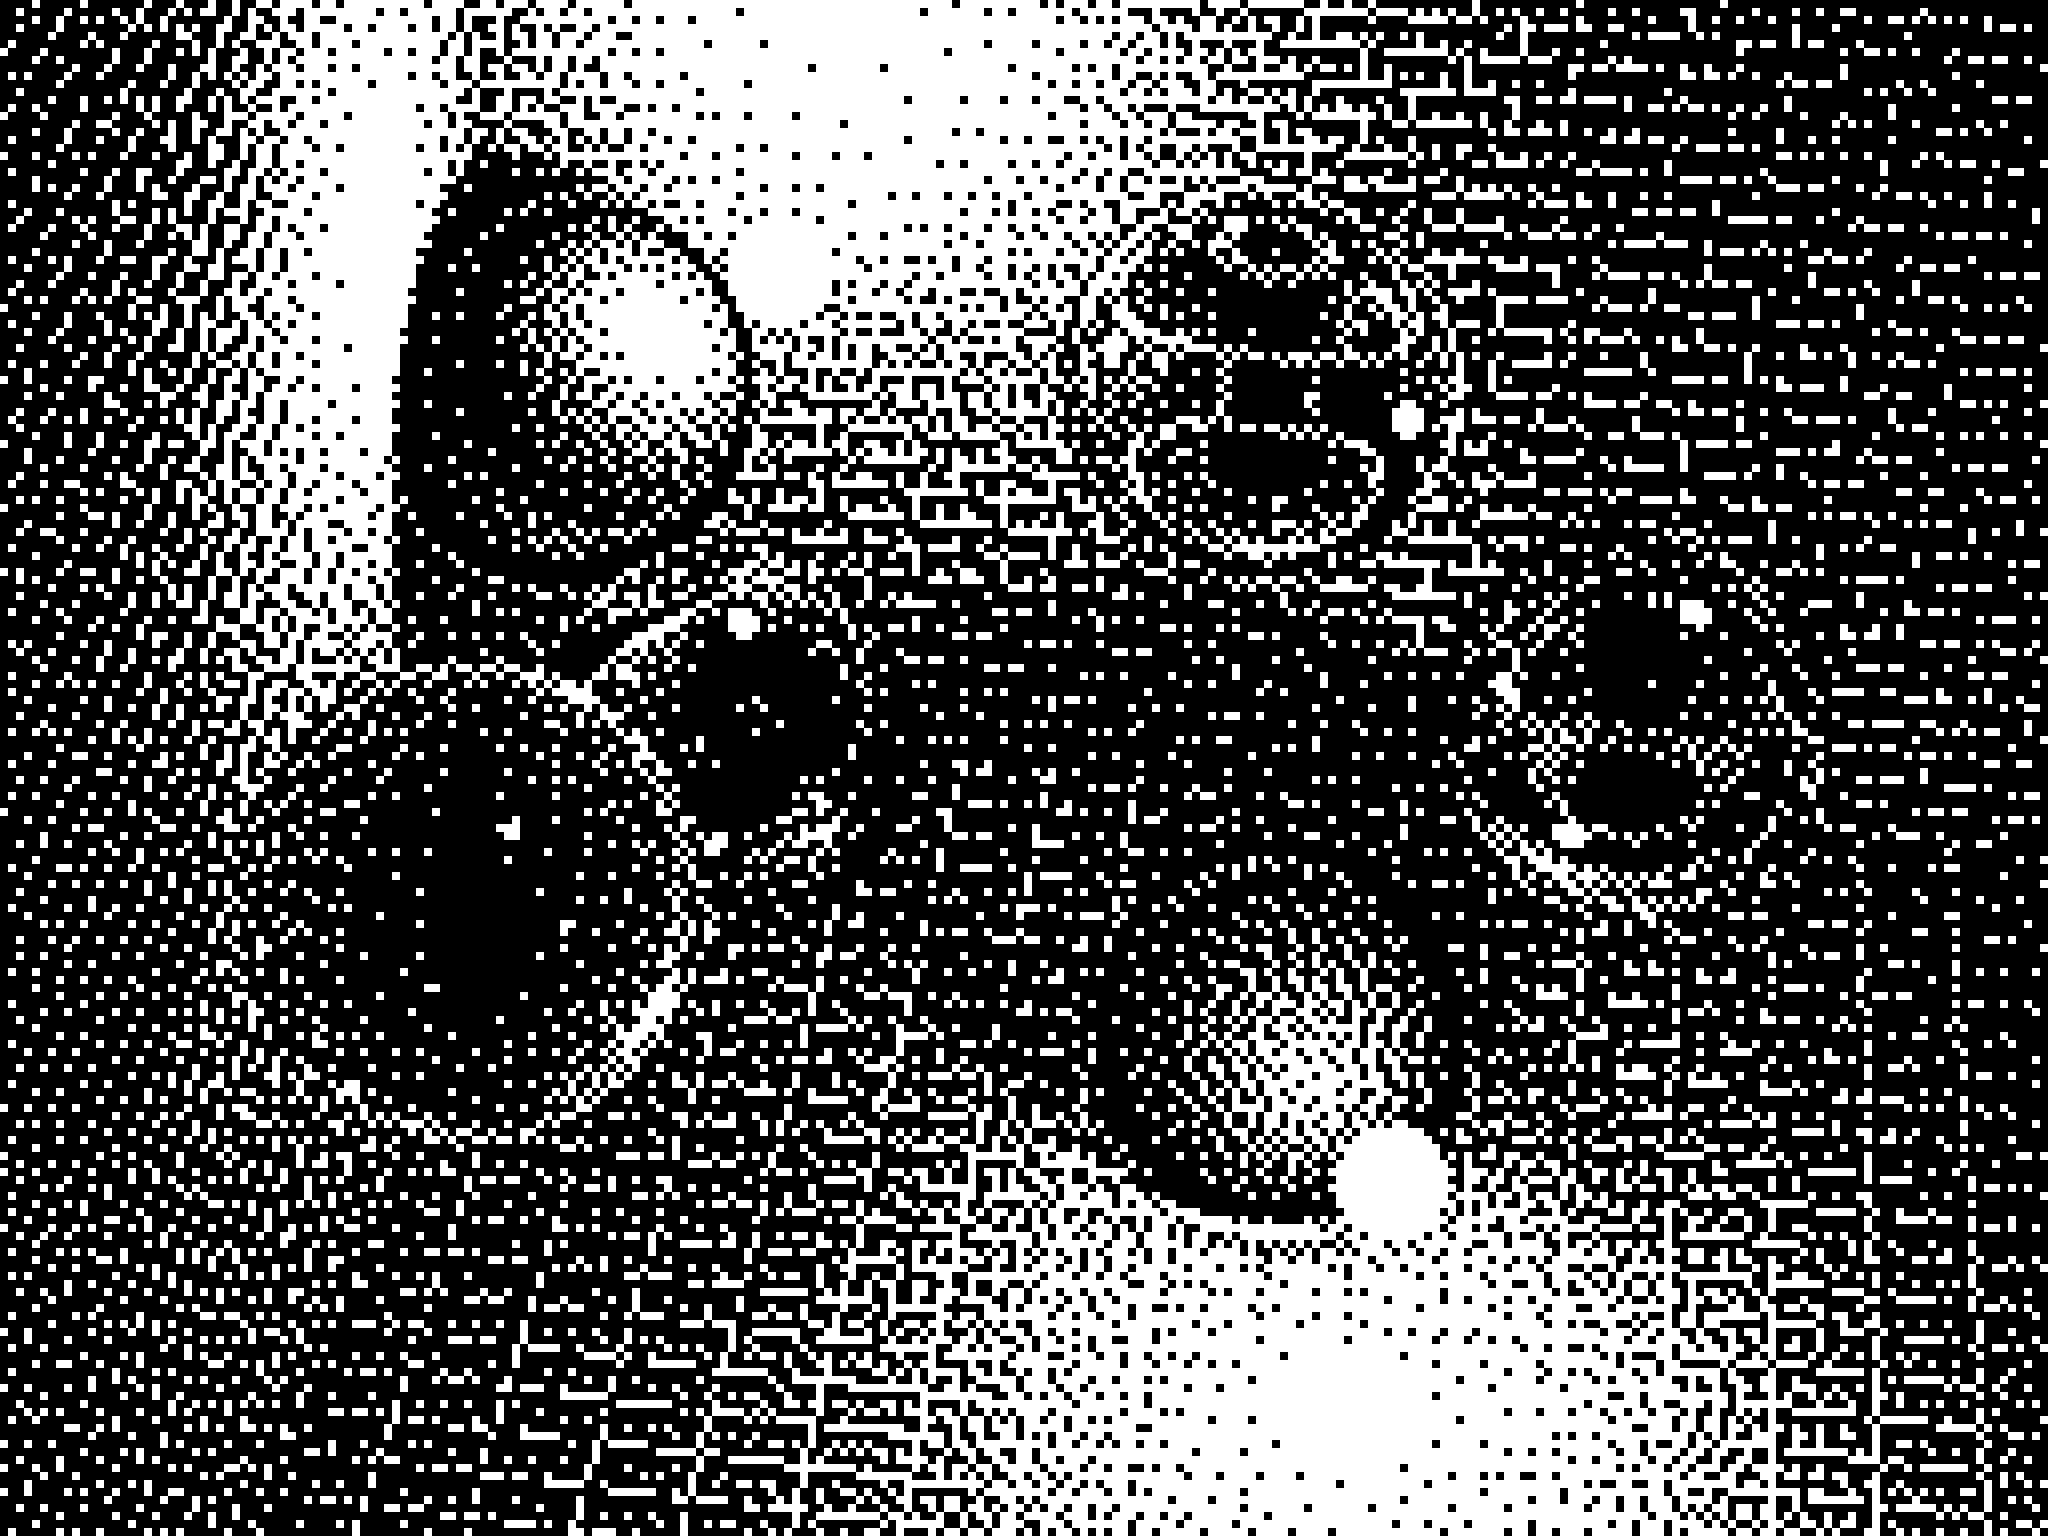
\includegraphics[width=1\textwidth]{logo.png}	\\
			\vspace{1cm}
			\Mail	\\
			\vspace{0.5cm}
			\textbf{\begin{LARGE} \Titolo \end{LARGE}}		\\
			\vspace{1cm}
			\textbf{Descrizione:} \Descrizione{}			\\
			\vspace{1cm}
			\begin{tabular}{ll}
				\textbf{Stato}               & \Stato              \\
				\textbf{Data}                & \Data               \\
				% forse è il caso di rimuovere redattori e verificatori, in modo
				% tale che un redattore oggi possa essere un verificatore
				% domani e viceversa. Inoltre, i documenti dovrebbero essere
				% scritti da ciascun componente del gruppo in momenti diversi
				\ifdefined\Redattori
					\midrule
				\textbf{Redattori}           & \Redattori          \\
				\textbf{Verificatori}        & \Verificatori       \\
				\fi

				\ifdefined\Approvatori
				\textbf{Approvatori}         & \Approvatori        \\
				\fi

				\ifdefined\ApprovatoriInterni
				\textbf{Approvatori interni} & \ApprovatoriInterni \\
				\fi

				\ifdefined\ApprovatoriEsterni
				\textbf{Approvatori esterni} & \ApprovatoriEsterni \\
				\fi

				\ifdefined\Destinatari
					\midrule
				\textbf{Destinatari}         & \Destinatari        \\
				\fi


				\ifdefined\Versione
					\midrule
				\textbf{Versione}            & \Versione           \\
				\fi
			\end{tabular}
		\end{center}
		\vspace{2cm}
		\ifdefined\Responsabile
		\begin{flushright}
			\begin{tabular}{ll}
				Il responsabile: & \Responsabile            \\
				                 &                          \\
				                 & \underline{\hspace{3cm}} \\
			\end{tabular}
		\end{flushright}
		\fi
	\end{titlepage}
	\newpage
}
